\section{John Joseph O'Brien}

\MainPerson{John Joseph\textsuperscript{3} O'Brien}\index{O'Brien!John Joseph\textsuperscript{3} (1861--1938)|bb} (\Lineage{2}{John}, \Lineage{1}{William}) was born in Boston, Suffolk County, Massachusetts,\index{Massachusetts!Boston} on 29 January 1861.\cite{John3OBrienBirth} He was baptized at St. John the Baptist Church\index{St.\ John the Baptist (church)} in Boston on 1 February 1861.\cite{John3OBrienBaptism} He died in Brookline, Norfolk County, Massachusetts,\index{Massachusetts!Brookline} on 15 May 1938.\cite{John3OBrienDeath} He is buried at Mt.\ Calvary Cemetery,\index{Mt.\ Calvary Cemetery} Boston.\cite{John3OBrienBurial} He married, at St. Augustine Church\index{St. Augustine (church)} in Boston on 6 February 1890, \MainPerson{Emma A.\ Mahony}.\index{Mahoney/Mahony!Emma}\index{O'Brien!Emma (Mahony)}\cite{John3OBrienMarriage,John3OBrienMarriage2} Emma was born in Boston\index{Massachusetts!Boston} on 27 September 1862 to Edward Mahony\index{Mahoney/Mahony!Edward} and Catherine Josephine Kenney.\index{Kenney!Catherine Josephine}\index{Mahoney/Mahony!Catherine Josephine (Kenney)}\cite{EmmaMahonyBaptism} She died in Brookline\index{Massachusetts!Brookline} on 11 July 1950.\cite{EmmaMahonyDeath}

John's father, John\textsuperscript{2},\index{O'Brien!John\textsuperscript{2}} died in 1863\cite{John2OBrienDeath} and his mother Mary\index{Mahoney/Mahony!Mary}\index{O'Brien!Mary (Mahoney)}\index{Bowser!Mary (Mahoney) (O'Brien)} married Thomas Bowser\index{Bowser!Thomas} in 1867.\cite{MaryMahoneyBowserMarriage} Sometime between 1870 and 1876, the family moved from Hanover St.\ in the North End\index{Massachusetts!Boston!North End}\index{Massachusetts!Boston!Hanover St.} to Hudson St.\ in Boston's South Cove neighborhood.\index{Massachusetts!Boston!Hudson St.}\index{Massachusetts!Boston!South Cove}\cite{ThomasBowser1870,ThomasBowser1876} The family later relocated to 45 Court St.\index{Massachusetts!Medford!45 Court St.} in Medford, Middlesex County, Massachusetts,\index{Massachusetts!Medford} and remained there for many years.\cite{Census1910John3OBrien,Census1930John3OBrien}

John worked as a picture frame manufacturer.\index{picture frame manufacturing}\index{frames|see{picture frame manufacturing}}  He took over the business from the previous owner, B.\ Ferdinand Sargent,\index{Sargent!B.\ Ferdinand} when Sargent relocated to Minnesota\index{Minnesota} in 1881 or 1882.\cite{PictureFrameLabel, Sargent} John continued running the business until about 1917.\cite{John3OBrien1916} The frame shop occupied the second floor of the building at 69 Cornhill\index{Massachusetts!Boston!Cornhill} in Boston.\cite{John3OBrien1916,FrameShopFire} 

\begin{figure}
\centering
\includegraphics[width=\textwidth]{picture_frames_label}
\caption{Label for John J.\ O'Brien,\index{O'Brien!John Joseph\string\textsuperscript{3} (1861--1938)|bb} picture frames,\index{picture frame manufacturing} 69 Cornhill, Boston, Mass., undated. Historic New England, Ephemera Collection, GUSN-265637 (\url{http://gusn.us/265637}).}
\end{figure}

\begin{figure}
	\centering
	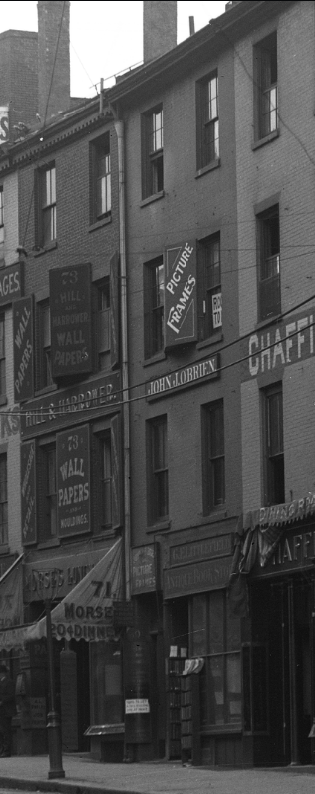
\includegraphics[height=0.8\textheight]{picture_frame_shop}
	\caption{John J.\ O'Brien's\index{O'Brien!John Joseph\string\textsuperscript{3} (1861--1938)|bb} frame shop\index{picture frame manufacturing} at 69 Cornhill, Boston.\index{Massachusetts!Boston!Cornhill} Detail from ``Crosswalk on Corn Hill opposite Franklin Avenue, looking west, sect. 8 1/2, Boston, Mass.,'' photograph, Boston Transit Commission, 14 Apr 1897, John Booras collection of plate glass negatives, Historic New England, GUSN-318238 (\url{http://gusn.us/318238}) }
\end{figure}

Cornhill\index{Massachusetts!Boston!Cornhill} was a street located at what is now the Government Center\index{Massachusetts!Boston!Government Center} complex. At its heyday, many booksellers\index{booksellers} and publishers located themselves on Cornhill and it became known as one of Boston's intellectual centers.\cite{Cornhill} The street was mostly destroyed during the city's urban renewal\index{urban renewal} phase in the 1960s. The only remnants of the original Cornhill are the Sears Block\index{Sears Block/Sears Crescent} and Sears Crescent (location of the famous ``steaming teakettle'').\cite{Cornhill}\index{steaming teakettle}

A fire\index{fire} in 1904 caused major damage to John's frame shop,\index{picture frame manufacturing} mostly from the water used to put out the fire. Efforts to fight the fire were complicated by an avalanche of snow falling off the roof and nearly burying the firefighters, and an intoxicated man trying to help by climbing the stairs of the building and hanging onto the firehose.\cite{FrameShopFire} John\index{O'Brien!John Joseph\textsuperscript{3} (1861--1938)|bb} was able to recover the business and continued operating out of this location until at least 1916.\cite{John3OBrien1916}

John,\index{O'Brien!John Joseph\textsuperscript{3} (1861--1938)|bb} his wife Emma,\index{Mahoney/Mahony!Emma}\index{O'Brien!Emma (Mahony)} and several of their children are buried in the Mahoney/Mahony plot owned by Emma's father Edward\index{Mahoney/Mahony!Edward} at Mt.\ Calvary Cemetery\index{Mt.\ Calvary Cemetery} in Boston's Roslindale\index{Massachusetts!Boston!Roslindale} neighborhood.\cite{John3OBrienBurial}

\begin{KidsIntro}
	Children of John Joseph\textsuperscript{3} O'Brien\index{O'Brien!John Joseph\textsuperscript{3} (1861--1938)|bb} and Emma A.\ (Mahony) O'Brien:\index{Mahoney/Mahony!Emma}\index{O'Brien!Emma (Mahony)}
\end{KidsIntro}

\begin{Kids}
	\KidNum{}{i.}\KidName{Mildred Loretta\textsuperscript{4} O'Brien},\index{O'Brien!Mildred Loretta\textsuperscript{4}} b.\ 14 Nov.\ 1890;\cite{Mildred4OBrienBirth} d.\ 26 May 1891.\cite{Mildred4OBrienDeath}
	
	\KidNum{\ref{per:Francis4OBrien}}{ii.}\KidName{Francis Joseph O'Brien},\index{O'Brien!Francis Joseph\textsuperscript{4}} b.\ 2 April 1892; m. Malden,\index{Massachusetts!Malden} Middlesex C., Mass., 12 Sept.\ 1921, \KidName{Mary Helena Flynn}.\index{Flynn!Mary Helena}\index{O'Brien!Mary Helena (Flynn)}
	
	\KidNum{\ref{per:Pauline4OBrien}}{iii.}\KidName{Pauline M.\ O'Brien},\index{O'Brien!Pauline M.\textsuperscript{4}}\index{Baine!Pauline M.\textsuperscript{4} (O'Brien)} b.\ 9 June 1894; m.\ 9 June 1930, \KidName{Charles Lucius Baine}.\index{Baine!Charles Lucius}
		
	\KidNum{\ref{per:Mildred4OBrien}}{iv.}\KidName{Mildred Louise O'Brien},\index{O'Brien!Mildred Louise\textsuperscript{4}}\index{French!Mildred Louise\textsuperscript{4} (O'Brien)} b.\ 29 Sept.\ 1896; m.\ Medford,\index{Massachusetts!Medford} Middlesex Co., Mass., Feb.\ 1925, \KidName{Albert Joseph French}.\index{French!Albert Joseph}
	
	\KidNum{}{v.}\KidName{Edward O'Brien},\index{O'Brien!Edward\textsuperscript{4} (1898--1898)} b.\ Medford,\index{Massachusetts!Medford} 5 July 1898;\cite{Edward4OBrienBirth} d.\ Medford, 24 Dec.\ 1898.\cite{Edward4OBrienDeath}
	
	\KidNum{}{vi.}\KidName{Almyra Louise O'Brien},\index{O'Brien!Almyra Louise\textsuperscript{4}} b.\ Medford, 27 June 1901;\cite{Almyra4OBrienBirth} d.\ Medford, 13 July 1902.\cite{Almyra4OBrienDeath}
\end{Kids}
